%&../.preamble
\endofdump

\usetikzlibrary{external}
\tikzset{external/system call={pdflatex --shell-escape --fmt=../.preamble --halt-on-error -jobname "\image" "\endofdump\texsource"}}
\tikzexternalize[prefix=tikz/]

\title{Introduction to ML}
\author{Marini Mattia}
\date{$ 3^o $ semestre $ 3^o $ anno}

\begin{document}
\maketitle
\tableofcontents
\newpage

\section{Gradient descent}
Per valutare la qualità di un modello, si usa una funzione di costo che misura la differenza fra i valori previsti e quelli reali. L'obiettivo è minimizzare questa funzione di costo.
\begin{definizione}{Funzione di loss}
	Una \textit{funzione di loss} è una funzione che misura la differenza tra i valori previsti e quelli reali.
\end{definizione}
Ad esempio, per un modello di classificazione lineare, la funzione di loss può essere il numero di punti che stanno dalla parte sbagliata del piano
\[
	\operatorname{loss}\left(w, b\right) = \sum_{i=1}^{n} 1\left[y_i \left(w\cdot x_i + b\right) < 0\right]
\]
l'obiettivo è minimizzare questa funzione ma spesso è molto difficile (NP-hard in fact). Spesso quindi si cerca un'approssimazione, cercando i minimi locali in funzioi che limitano la funzione di loss dall'alto:

\begin{definizione}{Funzione di loss surrogata}
	Una \textit{funzione di loss surrogata} è una funzione che approssima la funzione di loss, limitandola dall'alto.
\end{definizione}
Di seguito le seguenti funzioni di loss più comuni:
\begin{align*}
	\text{ 0-1 loss }         &  & \ell_{0/1}(y, y')            & = \mathbf{1}\bigl[y\,y' \le 0\bigr] \\
	\text{ hinge loss }       &  & \ell_{\mathrm{hinge}}(y, y') & = \max\bigl(0,\;1 - y\,y'\bigr)     \\
	\text{ exponential loss } &  & \ell_{\exp}(y, y')           & = \exp\bigl(-y\,y'\bigr)            \\
	\text{ square loss }      &  & \ell_{\mathrm{sq}}(y, y')    & = (y - y')^2
\end{align*}

Per trovare il minimo di una funzione di loss surrogata posso usare il \textit{gradient descent}, cercando di "scivolare" verso il minimo andando "in discesa" verso ogni asse singolarmente. Ad esempio utilizzando la loss function esponenziale
\[
	\operatorname{loss}\left(w, b\right) = \sum_{i=1}^{n} \exp \left(y_i \left(w\cdot x_i + b\right)\right)
\]
in particolare se cerco di modificare un peso alla volta considerando la loss function in una sola delle sue $ k $ dimensioni, ho che:
\begin{align*}
	w_j & = w_j - \eta \frac{d}{d w_j} \operatorname{loss}\left(w, b\right)            \\
	    & = w_j -\eta \sum_{i=1}^n -y_i x_{ij} \exp \left(-y_i (w\cdot x_i + b)\right)
\end{align*}

dunque abbiamo ottenuto la formula per aggiornare ciascun peso:
\[
	w_j = w_j +\eta \sum_{i=1}^n y_i x_{ij} \exp \left(-y_i (w\cdot x_i + b)\right)
\]
il che equivale a considerare ciascun punto nel training set e aggiornare il peso $ j $-esimo come segue:
\[
	w_j = w_j +\eta y_i x_{ij} \exp \left(-y_i (w\cdot x_i + b)\right) \quad \forall i \in \left[0,\ldots ,n\right]
\]

\begin{algoritmo}{Gradient descent}
	\begin{algorithm}[H]
		\KwIn{Learning rates $\eta = \left[\eta_1, \ldots \eta_n\right]$, loss function $ L $, \# of iterations $ K $}
		\KwOut{Weights $w = [w_1, \ldots, w_k]$}

		\vskip3mm
		\SetKwFunction{GD}{gradient\_descent}
		\Fn{\GD{$X, Y, L, \eta$}}{
			$ w ^{\left(0\right)} = \left[0,\ldots ,0\right] $ \Comment*{Dati come input in alternativa}
			\For{$ k \in \left[0, \ldots , K\right] $}{
				$ g^{\left(k\right)} = 	\nabla_{w^{\left(k\right)}} L $ \Comment*[r]{shift for each direction}
				$ w^{\left(k\right)} = w^{\left(k-1\right)} - \eta^{\left(k\right)} g^{\left(k\right)} $ \Comment*[r]{move in direction of gradient}
			}
			\Return $ w^{\left(k\right)} $
		}
	\end{algorithm}
\end{algoritmo}
Nota che $ w^{\left(k\right)} $ indica i pesi relativi alla $ k $-esima iterazione, ossia dopo essere stati migliorati $ k $ volte. Similmente $ g^{\left(k\right)} $ è il vettore contentente le derivate parziali (ossia considerate una direzione alla volta) della loss function nel punto ottenuto dopo $ k $ iterazioni:
\[
	\nabla_{w^{\left(k\right)}} L
	=
	\begin{bmatrix}
		\displaystyle \frac{\partial L}{\partial w_{1}^{\left(k\right)}} &
		\displaystyle \frac{\partial L}{\partial w_{2}^{\left(k\right)}} &
		\cdots                                                           &
		\displaystyle \frac{\partial L}{\partial w_{N}^{\left(k\right)}}
	\end{bmatrix}
\]
dove $ L $ è la \textit{funzione di loss}

\section{Unsupervised learning - riduzione dimensione}
L'idea generale è quella di "appirattire" i punti nell'asse parallela all'asse con varianza massima, così da ridurre al massimo la perdita di informazione
\vskip3mm
Formalmente si prende un versore $ w $ che parte da un punto $ c $. Un versore significa un vettore con norma 1, ossia
\[
	\left|w\right| = 1 \Leftrightarrow w^{T}w = 1
\]
dopodichè si condierano tutte le proiezioni dei punti $ x_i $ su questo versore, ossia
\[
	t_i = \left(x_i - c\right)^{T} w
\]

\subsubsection{Media e varianza}
La media serve per il calcolo della varianza, la quale è il criterio secondo cui eseguiamo la riduzione di dimensione:

\begin{align*}
	\mathbf{E}[t] & = \frac{1}{n} \sum_{i=1}^{n} t_i = \frac{1}{n} \sum_{i=1}^{n} (x_i - c)^\top w \\
	              & = \bar{x}^\top w - c^\top w
\end{align*}
dove
\[
	\bar{x} = \frac{1}{n} \sum_{i=1}^{n} x_i
\]


La varianza indica quanto i valori sono sparsi l'ungo l'asse identificato dal versore $ w $:
\begin{align*}
	\mathbf{Var}[t] & = \frac{1}{n} \sum_{i=1}^{n} (t_i - E[t])^2                                                    \\
	                & = \frac{1}{n} \sum_{i=1}^{n} \left[ x_i^\top w - c^\top w - \bar{x}^\top w + c^\top w\right]^2 \\
	                & = \frac{1}{n} \sum_{i=1}^{n} \left[ (x_i - \bar{x})^\top w \right]^2                           \\
	                & = \frac{1}{n} \sum_{i=1}^{n} \left( \bar{x}_i^\top w \right)^2                                 \\
	                & = \frac{1}{n} \sum_{i=1}^{n}  w^\top \bar{x}_i \bar{x}_i^\top w                                \\
	                & = w^\top \left[\frac{1}{n} \sum_{i=1}^{n}  \bar{x}_i \bar{x}_i^\top\right] w                   \\
	                & = w^\top \left[ \frac{1}{n} \bar{X} \bar{X}^\top \right] w                                     \\
	                & = w^\top C w
\end{align*}
dove
\begin{align*}
	t_i = \left(x_i - c\right)^{T}w &  & \bar{X} = \left[\bar{x_1}, \ldots , \bar{x_n}\right] &  & \bar{x_i} = \left(x_i - \bar{x}\right)
\end{align*}
e in particolare, $ C $ è della \textit{matrice della covarianza}
\vskip3mm
Dunque abbiamo ottenuto che la varianza è data da:
\[
	\mathbf{Var}[t] = w^\top C w
\]
dove $ C $ è la matrice della covarianza, definita come:
\[
	C =
	\begin{bmatrix}
		x_1 x_1 & \ldots & x_1 x_n \\
		x_2 x_1 &        & x_2 x_n \\
		\vdots  & \ddots & \vdots  \\
		x_n x_1 & \ldots & x_n x_n
	\end{bmatrix}
\]

\subsubsection{Autovalori e autovettori}
\begin{teorema}{Condizioni soluzione a sistema}
	Dato un sistema lineare nella forma $ Ax = 0 $, allora questo presenta soluzioni diverse da 0 se e solo se
	\[
		\operatorname{det}\left(A\right) = 0
	\]
\end{teorema}

\begin{definizione}{Autovettore e autovalore}
	Data una matrice $ A $ quadrata di dimensione $ n \times n $ allora $ x $ si dice un suo autovettore \textit{relativo al valore} $ \lambda  $ se vale che
	\[
		Ax = \lambda x
	\]
\end{definizione}
In particolare, per trovare autovettori e autovalori posso risolvere la seguente:
\[
	\operatorname{det}\left(A - \lambda I\right) = 0
\]
questo perchè:
\begin{align*}
	Av            & = \lambda v \\
	Av -\lambda v & = 0         \\
	\left(A - \lambda I \right) v = 0
\end{align*}
la quale ha soluzioni non nulle se e solo se $ \operatorname{det}\left(A - \lambda I\right) = 0 $
\begin{teorema}{Numero autovettori}
	Data una matrice quadrata di dimensione $ n \times n $, allora questa ha al massimo $ n $ autovettori linearmente indipendenti.
\end{teorema}

\begin{teorema}{Numero autovettori in matrice simmetrica}
	Data una matrice \underline{simmetrica} quadrata di dimensione $ n \times n $, allora questa ha \underline{esattamente} $ n $ autovettori linearmente indipendenti.
\end{teorema}

\subsubsection*{Decomposizione di matrici}
Data una matrice \( A \in \mathbb{R}^{m \times m} \) \underline{simmetrica}
\begin{itemize}
	\item Allora esiste \( U = [\mathbf{u}_1, \ldots, \mathbf{u}_m] \in \mathbb{R}^{m \times m} \) and
	      \( \boldsymbol{\lambda} = (\lambda_1, \ldots, \lambda_m)^\top \in \mathbb{R}^m \)

	      tale per cui:
	      \[
		      A = U \Lambda U^\top
	      \]
	      \begin{itemize}
		      \item $ U \in \R^{n \times n} $ una matrice che ha per colonne gli \textit{autovettori}
		      \item $ \Lambda \in \R^{n \times n} $ una matrice che ha sulla diagonale \textit{gli autovalori} ordinati
		      \item $U^\top U = UU^\top = I $
	      \end{itemize}

	\item O in alternativa
	      \[
		      A = \sum_{j=1}^m \lambda_j \mathbf{u}_j \mathbf{u}_j^\top
	      \]
	      \begin{itemize}
		      \item \( u_j \) autovettore
		      \item \( \lambda_j \) il corrispondente autovalore
	      \end{itemize}

	\item Nota che gli \textit{autovalori} vengono presi in ordine
	      \( \lambda_1 \geq \lambda_2 \geq \cdots \geq \lambda_m \)
\end{itemize}
\subsubsection{Obiettivo}
L'obbiettivo del nostro problema è trovare un sistema di riferimento in cui i il primo asse sia parallelo alla direzione con varianza massima, formalmente:
\[
	w_i = \operatorname{arg max} \left\{w ^{\top} C w :\; w ^{\top}w = 1, \quad w \perp w_j \quad \forall j : 1 \le j \le i<\right\}
\]

si può dimostrare che le la soluzione a questo problema di massimizzazione è dato dagli \textit{autovettori} di $ C $. In particolare, la $ i $-esima componente principale è data dall'$ i $-esimo autovettore di $ C $. Per trovare gli autovettori di $ C $ ho due metodi:
\vskip3mm
\sfblue{Eigenvalue decomposition}: data $ A \in \R^{m \times m} $ \textit{simmetrica} allora esiste
\begin{itemize}
	\item $ U = \left[u_1, \ldots , u_m\right] \in \R^{m \times m}$
	\item $ \lambda  = \left[\lambda_1, \ldots \lambda_m\right] $
\end{itemize}
tale per cui
\[
	A = U \Lambda U^\top
\]
dove
\[
	\Lambda = \begin{bmatrix}
		\lambda_1 &        &           \\
		          & \ddots &           \\
		          &        & \lambda_m
	\end{bmatrix}
\]
\vskip3mm
\sfblue{SVN (Singular Value Decomposition)}: data $ A \in \R^{m \times n} $, allora esistono:
\begin{itemize}
	\item $ U  = \left[u_1, \ldots , u_m\right]\in  \R^{m \times k} $
	\item $ s = \left[s_1, \ldots , s_n\right] \in \R^{k} $
\end{itemize}
tali per cui
\[
	A = USV^{\top}
\]
dove
\[
	\Lambda = \begin{bmatrix}
		s_1 &        &     \\
		    & \ddots &     \\
		    &        & s_m
	\end{bmatrix}
\]

\subsubsection{Equivalenza metodi:}
Dato il fatto che $ C = \frac{1}{n} \bar{X}\bar{X}^{\top} $, allora posso
\begin{itemize}
	\item Chiamare $ U, \lambda = \operatorname{eig}\left(C\right) $
	\item Chiamare $ U, s, V = \operatorname{SVN}\left(\bar{X}\right) $ e calcolare
	      \[
		      \lambda = \left[\frac{\lambda_1 ^2}{n}, \ldots , \frac{\lambda_n ^2}{n}\right]
	      \]
\end{itemize}
L'equivalenza dei due metodi è data dal fatto che:
\[
	C = \frac{1}{n} \bar{X}\bar{X}^{\top} = \frac{1}{n} USV \left(USV\right)^{\top}= \frac{1}{n}\left(USV\right) \left(V^\top S^\top U^\top\right) = \frac{1}{n} U S^2 U^{\top}
\]
quindi
\[
	C =  \frac{1}{n} U S^2 U^{\top}
\]

\subsubsection{Pseudocodice}



\begin{algoritmo}{PCA with eigenvalue decomposition}
	\begin{algorithm}[H]
		\KwIn{Data points $X = [x_1, \ldots, x_n]$}
		\KwOut{Principal components $U = [u_1, \ldots, u_m], \lambda = [\lambda_1, \ldots, \lambda_m]$}
		\vskip3mm

		\SetKwFunction{PCAeig}{pca\_eigen}
		\SetKwFunction{eig}{eig}
		\Fn{\PCAeig{$X$}}{
		\vskip3mm
		\Comment{Centring points}
		$ \bar{X} = X - \frac{1}{n} X 1_n 1_n^{\top}$\;

		\vskip3mm
		\Comment{Compute covariance matrix}
		$C = \frac{1}{n} \bar{X} \bar{X}^{\top}$\;

		\vskip3mm
		\Comment{Eigenvalue decomposition}
		$U, \lambda$ = \eig{$C$}\;

		\vskip3mm
		\Return{$ U, \lambda $}\;
		}
	\end{algorithm}
	dove $ 1_n $ è un vettore \textit{colonna} di dimensione $ n $ con tutti gli elementi uguali a 1.
\end{algoritmo}

\begin{algoritmo}{PCA with SVD}
	\begin{algorithm}[H]
		\KwIn{Data points $X = [x_1, \ldots, x_n]$}
		\KwOut{Principal components $U = [u_1, \ldots, u_k], \lambda = \left[\lambda_1, \ldots , \lambda _n\right]$}
		\vskip3mm

		\SetKwFunction{PCA}{pca\_svd}
		\SetKwFunction{SVD}{svd}
		\Fn{\PCA{$X$}}{
		\vskip3mm
		\Comment{Centring points}
		$ \bar{X} = X - \frac{1}{n} X 1_n 1_n^{\top}$\;

		\vskip3mm
		\Comment{SVN decomposition}
		$U, s, V$ = \SVD{$ \bar{X} $}\;

		\vskip3mm
		\Comment{Computing $ \lambda $}
		$ \lambda = \left( \frac{s_1^2}{n}, \ldots, \frac{s_k^2}{n} \right)$\;

		\vskip3mm
		\Return{$ U, \lambda $}\;
		}
	\end{algorithm}
	dove $ 1_n $ è un vettore \textit{colonna} di dimensione $ n $ con tutti gli elementi uguali a 1.
\end{algoritmo}
\vskip3mm
Nota che per ridurre le dimensioni dei valori di un qualsiasi campione è sufficiente trovare la sua proiezione sulle componenti principali. Ricordando che la proiezione di $ b $ su $ a $ è data da $ a \cdot b  = a^{\top} b$, possiamo generalizzare al nostro caso.
\vskip3mm
Dato $ \hat{W} = \left[w_1, \ldots ,w_k\right] $ contente le componenti principali e $ \bar{X}\left[x_1, \ldots ,x_n\right] $ contenente i campioni da proiettare, allora
\[
	T = \hat{W}^{\top} \bar{X}
\]
$ T $ ha \textit{come colonne} le proiezioni dei campioni sulle componenti principali

\subsubsection{Trovare di quanto ridurre}
Al fine di trovare un numero di dimensioni oppurtuno per cui si vuole effettura la riduzione è possibile stimare la quantità di informazione persa con le sguenti formule:
\vskip3mm
\begin{minipage}[t]{0.48\textwidth}
	\begin{center}
		\[
			\frac{\sum_{j=1}^k \lambda_j}{\sum_{j=1}^m C_{jj}}
		\]
		Eigenvalue decomposition
	\end{center}
\end{minipage}
%
\begin{minipage}[t]{0.48\textwidth}
	\begin{center}
		\[
			\frac{\sum_{j=1}^k s_j^2}{\sum_{ij} \bar{X}_{ji}^2}
		\]
		Singular value decomposition
	\end{center}
\end{minipage}
\vskip3mm
queste due formule stimano la percentuale di informazione che viene ritenuta dopo aver ridotto la dimensione a $ k $.

\section{Clustering}
\subsection{k-means}
\begin{itemize}
	\item Dati dei punti $X = [x_1, \ldots, x_n] \in \mathbb{R}^{d \times n}$
	\item Impostato un numero di \textit{cluster} $k$
	\item Partiziona i punti in $k$ cluster minimizzando la \textit{variazione} totale
	      \[
		      \min_{\mathcal{C}_1, \ldots, \mathcal{C}_k} \sum_{j=1}^k V(\mathcal{C}_j)
	      \]
	\item La variazione all'interno di un cluster $ \mathcal{C}_j $ è definita come
	      \[
		      V(\mathcal{C}_j) = \sum_{i \in \mathcal{C}_j} \| x_i - \mu_j \|^2
	      \]
	\item Il centroide è solitamente dato dal "centro di massa" fra i punti:
	      \[
		      \mu_j = \frac{1}{|\mathcal{C}_j|} \sum_{i \in \mathcal{C}_j} x_i
	      \]
\end{itemize}
\subsubsection{Pseudocodice}

\begin{algoritmo}{k-means}
	\begin{algorithm}[H]
		\SetKwFunction{kclustering}{k\_clustering}
		\Fn{\kclustering{$ X $}}{
			\Comment{Initialization strategy to get initial cluster centroids $\mu_1, \ldots, \mu_k$}
			\While{clusters change}{
				\For{ $x_i \in X$}{
					Assign $x_i$ to the closest centroid, i.e.\\
					$
						\mathcal{C}_j = \left\{ i \in \{1, \ldots, n\} : j = \arg\min_\ell \| x_i - \mu_\ell \| \right\}
					$
				}
				Compute new cluster centroids $\mu_1, \ldots, \mu_k$\;
			}
			\Return{$ \mathcal{C}_1, \ldots, \mathcal{C}_k $}\;
		}
	\end{algorithm}
\end{algoritmo}
\subsubsection{Note}
\begin{itemize}
	\item Algoritmo termina sempre, ma potrebbe finire in \textit{minimo locale}, non globale. La \textit{loss function} non è convessa
	\item Risultati variano molto in base a come si scelgono i cluster iniziali. I metodi più comuni sono:
	      \begin{itemize}
		      \item Random points (not examples) in the space
		      \item Randomly pick examples
		      \item Points least similar to any existing center (furthest centers heuristic)
		      \item Try out multiple starting points
		      \item Initialize with the results of another clustering method
	      \end{itemize}
	\item Complessità ad ogni iterazione:
	      \begin{itemize}
		      \item $ O\left(k n\right) $ per assegnare ognuno degli $ n $ punti ad un cluster $ k $
		      \item $ O\left(n\right) $ computazione centroidi
	      \end{itemize}
	\item Talvolta la distanza euclidea è poco adeguata, vedi \cref{cosine-distance}
	\item L'assunzione di base sulla distribuzione dei dati è che questi siano disposti in maniera "sferica" (generizzabile a più dimensioni)
\end{itemize}

\subsection{EM-clustering}
L'EM assume che i dati provengano da una \textbf{miscela di distribuzioni gaussiane} (invece di cluster sferici come K-means). Ogni cluster è rappresentato da una gaussiana che può avere forma ellittica, permettendo di catturare cluster con forme più complesse.

\begin{itemize}
	\item A differenza del K-means (assegnazione \textit{hard}), qui un punto può appartenere a più cluster con probabilità diverse
	\item Ad esempio un punto può avere probabilità $p(\text{rosso}) = 0.8$ e $p(\text{blu}) = 0.2$
\end{itemize}

\vskip3mm
L'algoritmo alterna tra due passi principali:
\begin{itemize}
	\item Per ogni punto $x_i$, calcola la \textit{probabilità} $p(\theta_c | x_i)$ che appartenga a ciascun cluster $c$
	\item Ricalcola i parametri $\theta_c$ di ogni cluster (centro $\mu_c$ e matrice di covarianza $\Sigma_c$) usando le probabilità calcolate nel passo precedente
	\item Ogni punto contribuisce al nuovo centro in modo \textit{pesato} secondo la sua probabilità di appartenenza
\end{itemize}




L'algoritmo continua ad alternare i due passi fino a convergenza:

\begin{align}
	\text{E-step: } & \quad p(\theta_c | x_i) = \frac{p(x_i | \theta_c) p(\theta_c)}{\sum_{j=1}^{K} p(x_i | \theta_j) p(\theta_j)}                              \\[0.5em]
	\text{M-step: } & \quad \theta_c^{(\text{new})} = \arg\max_{\theta_c} \sum_{i=1}^{N} p(\theta_c | x_i) \log p(x_i | \theta_c) \label{em-clustering-formule}
\end{align}

L'algoritmo garantisce che la likelihood dei dati aumenti ad ogni iterazione (anche se può convergere a un ottimo locale).

\vskip3mm
Nota: $ p\left(x_i \mid \theta_c\right) $ è la funzione gaussiana valutata in $ x_i $. La generalizzazione della gaussiana in $ d $ dimensioni è:
\[
	\mathcal{N}[x; \mu, \Sigma] = \frac{1}{(2\pi)^{d/2} \sqrt{\det(\Sigma)}} \exp\left[-\frac{1}{2}(x - \mu)^T \Sigma^{-1} (x - \mu)\right]
\]
dove $ \Sigma  $ è la \textit{matrice di covarianza} che descrive la forma dell'ellisse del cluster e $ \mu  $ è la \textit{media}

\subsection{Specteal clustering}
Lo spectral clustering può aiutare nel momento in cui i dati non sono distribuiti in maniera gaussiana o circolare. L'algoritmo funziona così:
\begin{itemize}
	\item Costruzione grafo secondo qualche criterio
	\item Partizione del grafo minimizzando il peso del taglio, ossia
	      \[
		      \operatorname{cut}\left(A, B\right) = \sum_{x \in A, y \in B} w\left(x,y\right)
	      \]
	      più nello specifico, si cerca di minimizzare il taglio normalizzato:
	      \[
		      \operatorname{Ncut}\left(A,B\right) = \frac{\operatorname{cut}\left(A,B\right)}{\operatorname{vol}\left(A\right)} + \frac{\operatorname{cut}\left(A,B\right)}{\operatorname{vol}\left(B\right)}
	      \]
	      nota che il taglio va \textit{normalizzato} per evitare che il taglio sia influenzato dalla dimensione dei cluster, evitando tagli in cui ho 99 nodi da una parte e 1 dall'altra
\end{itemize}
Il problema può essere generalizzato ad un problema di autovalori

\subsection{Clustering gerarchico}
L'idea del clustering gerarchico è di procedere in maniera \textit{agglomerativa} e \textit{bottom-up}, aggregando gruppi simili
\begin{itemize}
	\item Ogni elemento $ \xi  $ è inizialmente un cluster
	\item Unisco gruppi secondo qualche criterio
	\item Termino quando rimane un singolo cluster
\end{itemize}
La struttura gerarchica ottenuta è detta \textit{dendogramma}
\vskip3mm
Ciò che caratterizza un algoritmo è proprio come si definisce la distanza fra clusters. Ci sono molte opzioni quali: closest pair, farest pair, average among all distances, etc


\subsubsection{Pseudocodice}
Formalmente, per risolvere il problema decsritto in \cref{em-clustering-formule}, è necessario procedere come segue:
\begin{align*}
	N_c      & = \sum_{i = 0}^{k} p\left(x \mid \theta_c\right)                                                  \\
	\Sigma_c & = \frac{1}{N_c} + \sum_{i=1}^{n} p\left(\theta_c \mid x_i\right) \cdot \bar{x_i} \bar{x_i}^{\top} \\
	\pi_c    & = p\left(\theta_c\right)  = \frac{N_c}{n}
\end{align*}

\begin{algoritmo}{EM-clustering}
	\begin{algorithm}[H]
		\KwIn{Data points $X = [x_1, \ldots, x_n] \in \mathbb{R}^{d \times n}$, number of clusters $K$}
		\KwOut{$ K $ clusters with parameters $ \theta_c = (\mu_c, \Sigma_c, \pi_c) $}
		\SetKwFunction{emclustering}{em\_clustering}

		\vskip3mm
		\Fn{\emclustering{$ X, K $}}{
			\Comment{Inizializzo $ \pi $}
			\For{$ c \in K $}{
				$ \pi_i = \frac{1}{k} $
			}

			\vskip3mm
			\While{clusters change}{
				\Comment{E-step: calcolo le probabilità di appartenenza}
				\For{$ c \in K $}{
					$\displaystyle \gamma_{iC} = p\left(\theta_c, \xi \right) = \frac{p(x_i | \theta_c) p(\theta_c)}{\sum_{j=1}^{K} p(x_i | \theta_j) p(\theta_j)} $\;
				}

				\vskip3mm
				\Comment{M-step: aggiorno gaussian parameters}

				\For{$ c \in K $}{
					$\displaystyle N_c       = \sum_{i = 0}^{k} p\left(x \mid \theta_c\right)$\;
					$\displaystyle \Sigma_c  = \frac{1}{N_c} + \sum_{i=1}^{n} p\left(\theta_c \mid x_i\right) \cdot \bar{x_i} \bar{x_i}^{\top} $\;
					$\displaystyle \pi_c     = p\left(\theta_c\right)  = \frac{N_c}{n}$\;
				}
			}
		}
	\end{algorithm}
\end{algoritmo}



\subsubsection{Vantaggi rispetto a k-means}
\begin{enumerate}
	\item \textit{Cluster ellittici}: Può gestire cluster con forme allungate, non solo circolari
	\item \textit{Clustering soft}: Fornisce probabilità di appartenenza invece di assegnazioni rigide
	\item \textit{Maggiore flessibilità}: La matrice di covarianza permette di catturare correlazioni tra le features
\end{enumerate}

\section{Reti neurali}

\begin{center}
	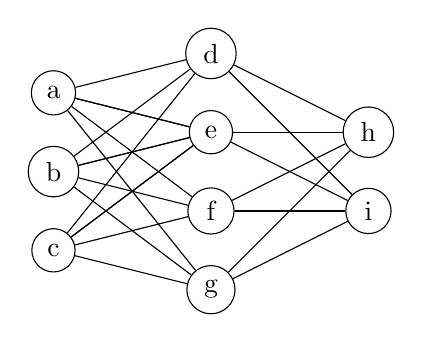
\begin{tikzpicture}
		\node (a)[draw, circle] at (0, 1)   {a};
		\node (b)[draw, circle] at (0, 0)   {b};
		\node (c)[draw, circle] at (0,-1)  {c};

		\node (d)[draw, circle] at (2, 1.5)   {d};
		\node (e)[draw, circle] at (2, 0.5)   {e};
		\node (f)[draw, circle] at (2,-0.5)   {f};
		\node (g)[draw, circle] at (2,-1.5)   {g};

		\node (h)[draw, circle] at (4, 0.5)   {h};
		\node (i)[draw, circle] at (4,-0.5)   {i};

		\draw (a)edge(d)edge(e)edge(e)edge(f)edge(g);
		\draw (b)edge(d)edge(e)edge(e)edge(f)edge(g);
		\draw (c)edge(d)edge(e)edge(e)edge(f)edge(g);

		\draw (d)edge(h)edge(i);
		\draw (e)edge(h)edge(i);
		\draw (f)edge(h)edge(i);
		\draw (g)edge(h)edge(i);
	\end{tikzpicture}
\end{center}

\subsection{Calcolo output predetto}
Data una rete neurale con $ L $ layers, l'idea è che ogni nodo ha un'attivazione, ogni edge un peso. Per calcolare l'attivazione di un nodo $ t $ devo fare una "somma pesata" di tutti i nodi ai quali è collegato $ t $.

\begin{center}
	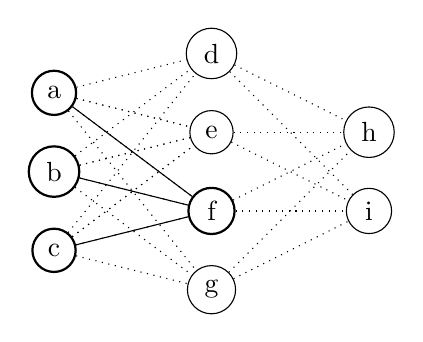
\begin{tikzpicture}
		\node (a)[draw, circle, thick] at (0, 1)   {a};
		\node (b)[draw, circle, thick] at (0, 0)   {b};
		\node (c)[draw, circle, thick] at (0,-1)  {c};

		\node (d)[draw, circle] at (2, 1.5)   {d};
		\node (e)[draw, circle] at (2, 0.5)   {e};
		\node (f)[draw, circle, thick] at (2,-0.5)   {f};
		\node (g)[draw, circle] at (2,-1.5)   {g};

		\node (h)[draw, circle] at (4, 0.5)   {h};
		\node (i)[draw, circle] at (4,-0.5)   {i};

		\draw [dotted](a)edge(d)edge(e)edge(e)edge(f)edge(g);
		\draw [dotted](b)edge(d)edge(e)edge(e)edge(f)edge(g);
		\draw [dotted](c)edge(d)edge(e)edge(e)edge(f)edge(g);

		\draw [dotted](d)edge(h)edge(i);
		\draw [dotted](e)edge(h)edge(i);
		\draw [dotted](f)edge(h)edge(i);
		\draw [dotted](g)edge(h)edge(i);

		\draw (f)edge(a)edge(b)edge(c);
	\end{tikzpicture}
\end{center}
in questo caso:
\[
	\text{ Attizazione di $ f $ } = h(z_f = z_a + w_{af} + z_b + w_{bf} + z_c + w_{cf} + b_f)
\]
dove $ b_f $ è il bias di f e $ h $ è la funzione di attivazione. In termini generali:
\[
	z_t = \sum_{i \in \mathcal{N}(t)} w_{it} z_i + b_t
\]
\subsubsection{Classicifazione: softmax + cross-entropy}
Una volta calcolate le attivazioni dell'ultimo layer per confrontarle con il risultato atteso ($ y $) posso procedere come segue. Supponendo di avere
\begin{center}
	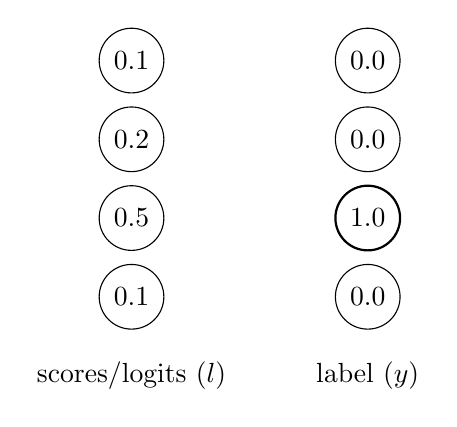
\begin{tikzpicture}
		\node ()[draw, circle] at (0,0)  {0.1};
		\node ()[draw, circle] at (0,1)  {0.5};
		\node ()[draw, circle] at (0,2)  {0.2};
		\node ()[draw, circle] at (0,3)  {0.1};
		\node ()[] at (0,-1)  {scores/logits ($ l $)};

		\node ()[draw, circle] at (3,0)  {0.0};
		\node ()[draw, circle, thick] at (3,1)  {1.0};
		\node ()[draw, circle] at (3,2)  {0.0};
		\node ()[draw, circle] at (3,3)  {0.0};
		\node ()[] at (3,-1)  {label ($ y $)};
	\end{tikzpicture}
\end{center}
\sfblue{Softmax}: la funzione \textit{softmax} è definita come:
\[
	\operatorname{softmax}\left(l\right) = S\left(l\right) = \frac{\exp\left(l_i\right)}{\sum_{j=1}^{k} \exp\left(l_j\right)}
\]
intuitivamente:
\begin{itemize}
	\item Applica esponenziale a ogni score $ z_i $ per enfatizzare gli outliers
	\item Normalizza il vettore $ l $ rendendolo una distribuzione di probabilità
\end{itemize}
questo equivale a creare il vettore:
\[
	S\left(l\right) = \left[\frac{e^{l_1}}{\sum_{j} e^{l_j}}, \ldots , \frac{e^{l_m}}{\sum_{j} e^{l_j}}\right]
\]

\vskip3mm
\sfblue{Cross-entropy loss}: la \textit{cross-entropy} è definita come:
\[
	\operatorname{cross-entropy}\left(l, y\right) = \mathcal{L}\left(l,y\right) = \sum_{k} y_k \log \left(S\left(l_k\right)\right)
\]

In termini vettoriali, dato $ l $ il vettore degli score e $ y $ ossia la label che indica il risultato atteso, allora la \textit{cross-entropy} è definita come:
\[
	\mathcal{L}\left(l, y\right) = S(l)^{\top}y
\]





\sfblue{Esempio}: nel nostro caso:
\[
	S \left(l\right) = S\left(\left[0.1,0.2, 0.5, 0.1\right]\right) = \frac{1}{\sum_{j} e^{j}} \left[e^{0.1}, e^{0.2}, e^{0.5}, e^{0.1}\right]
\]
calcolo la sommatoria:
\[
	\sum_i e^{l_i} = e^{0.1} + e^{0.2} + e^{0.5} + e^{0.1} \approx 3.2
\]
dunque
\[
	S\left(l\right) = \frac{1}{3.2} \left[ 1.1, 1.2, 1.6, 1.1\right] \approx \left[ 0.34, 0.38, 0.5, 0.34 \right]
\]

\subsubsection{Regressione: softmax + cross-entropy}
Se il vettore $ l $ degli scores deve dare origine ad una regressione di $ n $ valori allora posso calcolare la distanza dal valore atteso $ \hat{y} $ con la loss quadratica:
\[
	\mathcal{L}\left(l, \hat{y}\right) = \frac{1}{2} \sum_{i=1}^{n} \left(l_i - \hat{y}_i\right)^2
\]
nota che questa loos function è relativa \textit{al singolo input $ x_i $}


\vskip3mm
\section{Miscellanea nozioni}
\subsection{Cosine distance}\label{cosine-distance}
In alcuni casi la distanza euclidea non è adeguata per valutare quanto due vettori sono simili. Ad esempio, se classificassimo documenti sulla base delle parole contenute e avessimo:

\begin{center}
	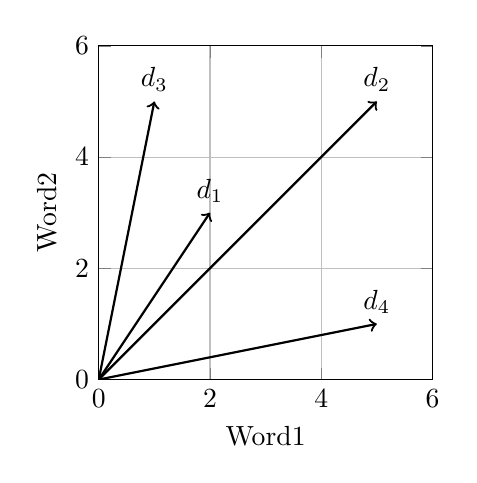
\begin{tikzpicture}
		\begin{axis}[
				xmin=0, xmax=6,
				ymin=0,ymax=6,
				width=0.48\textwidth, height=0.48\textwidth, grid=major,   ylabel=Word2, xlabel=Word1]
			\draw [thick, ->](0,0)--(2,3) node [above] {$ d_1 $};
			\draw [thick, ->](0,0)--(5,5) node [above] {$ d_2 $};
			\draw [thick, ->](0,0)--(1,5) node [above] {$ d_3 $};
			\draw [thick, ->](0,0)--(5,1) node [above] {$ d_4 $};
		\end{axis}
	\end{tikzpicture}
\end{center}
in questo caso $ d_1 $ e $ d_2 $ sono molto distanti mentre dal punto di vista logico risultano molto simili. Per questo è più efficiente la \textit{cosine similarity}
\[
	\operatorname{sim} \left(x,y\right) = \frac{x}{\left|\left|x\right|\right|}\cdot  \frac{y}{\left|\left|y\right|\right|}
\]
nota come $ \operatorname{sim}\left(x,y\right) \in \left[0,1\right] $. Similmente:

\[
	\operatorname{d\left(x,y\right)} = 1 - \operatorname{sim}\left(x,y\right)
\]





\end{document}
